\documentclass[12pt]{article}
\usepackage[a4paper, left=3.5cm, right=1.25cm, top=2.5cm, bottom=1.25cm]{geometry}
\usepackage{newtxtext}
\usepackage{graphicx}
\usepackage{enumitem}
\usepackage{cite}   % improves citation formatting
\usepackage{url}    % handles URLs safely
\usepackage{setspace}



\begin{document}
\begin{center}

%\vspace*{1.2cm}

% Project Title
{\fontsize{24pt}{28pt}\selectfont \textbf{BLOCKCHAIN SECURE VAULT}}\\[1.2cm]

% Project Synopsis
{\fontsize{14pt}{18pt}\selectfont \textbf{PROJECT SYNOPSIS}}\\[0.8cm]

% Minor Project
{\fontsize{12pt}{14pt}\selectfont OF MINOR PROJECT}\\[1.5cm]

% Degree
{\fontsize{14pt}{18pt}\selectfont \textbf{BACHELOR OF TECHNOLOGY}}\\[1cm]

% Branch
{\fontsize{16pt}{20pt}\selectfont Computer Science Engineering}\\[1.8cm]

% Submitted By
{\fontsize{12pt}{14pt}\selectfont SUBMITTED BY}\\[0.6cm]

% Student Name

{\fontsize{14pt}{18pt}\selectfont EKAMPREET SINGH \hfill 2302515}\\[0.6cm]
{\fontsize{14pt}{18pt}\selectfont GAURAV PRASHAR\hfill 2302518}\\[0.6cm]
{\fontsize{14pt}{18pt}\selectfont GAURAV SHARMA\hfill 2302519}\\[1.5cm]

% Month & Year
{\fontsize{12pt}{14pt}\selectfont January 2026}\\[1.8cm]

% College Logo

\includegraphics[width=4cm]{gne_logo.png}\\[1cm]

% College Name
{\fontsize{16pt}{20pt}\selectfont \textbf{GURU NANAK DEV ENGINEERING COLLEGE,}}\\[0.3cm]
{\fontsize{16pt}{20pt}\selectfont \textbf{LUDHIANA}}

\vspace*{1cm}

\end{center}
\newpage
\begin{abstract}
\doublespacing
Blockchain Secure Document Vault is a trustless document management system that integrates end-to-end encryption, decentralized storage, and blockchain-based integrity verification. The platform addresses critical limitations of centralized cloud storage solutions by enabling organizations operating in compliance-intensive sectors such as legal, healthcare, and finance to maintain complete control over document security while generating immutable proof of file integrity and access history.

The system follows a hybrid architecture in which documents are encrypted locally using the AES-256 encryption standard and hashed using the SHA-256 algorithm. Encrypted files are stored on the InterPlanetary File System (IPFS) to ensure decentralized availability, while cryptographic integrity hashes are committed to a blockchain ledger to provide tamper-proof verification. Users retain full ownership of cryptographic keys, ensuring a trustless security model, while benefiting from a transparent and verifiable audit trail that reduces reliance on manual compliance audits.

The technology stack includes Next.js and React for the frontend, Node.js with Express and MongoDB for backend services, Solidity-based smart contracts for integrity proofs, and IPFS for distributed storage. The project has been fully developed and tested, achieving stable performance and secure operation, making it suitable for real-world deployment.
\end{abstract}
\newpage
\tableofcontents
\newpage


\newpage
\section{Introduction}

\subsection{Brief introduction about the project to be developed}

This project presents a secure and user-friendly platform for document storage with verifiable integrity. Conventional cloud storage solutions often prioritize convenience over security, leading to risks related to confidentiality and undetectable tampering \cite{stallings2017}. To overcome these limitations, the proposed system integrates end-to-end encryption with blockchain-based verification, ensuring that documents remain private while their authenticity can be independently validated.

Users can securely register, upload encrypted documents, and verify file integrity by comparing cryptographic hashes with immutable on-chain records. A modern web interface, combined with a robust backend, manages encryption, access control, and secure sharing workflows. The system aims to make strong security practices and trustworthy document verification accessible to individuals and organizations without requiring specialized expertise.

\subsection{Technology Used}
\begin{itemize}
\item \textbf{Frontend:} Next.js with TypeScript
\item \textbf{Backend:} Node.js and Express for REST APIs, authentication, and file handling
\item \textbf{Blockchain:} Solidity smart contracts using Hardhat for on-chain hash storage and verification
\item \textbf{Cryptography:} AES-256 for encryption and SHA-256 for hashing \cite{nist197}
\item \textbf{File Processing:} Mammoth.js for DOCX files, PDF.js for PDF rendering, and Web Crypto API for client-side decryption
\end{itemize}

\subsection{Field of Project}
\begin{itemize}
\item Information Security and Web Application Development
\item Blockchain-based Integrity Verification
\item Secure and Compliance-Oriented Document Management
\end{itemize}

\subsection{Special Technical Terms}
\begin{itemize}
\item \textbf{End-to-End Encryption (E2EE):} Files are encrypted before upload and decrypted only by authorized users.
\item \textbf{Content Hash:} A cryptographic fingerprint used to detect file modifications.
\item \textbf{On-chain Verification:} Validation of file integrity using immutable blockchain records.
\item \textbf{Smart Contract:} Blockchain program that stores and exposes document hashes.
\item \textbf{Immutable Ledger:} Tamper-resistant blockchain record ensuring data integrity.
\end{itemize}


\newpage
\section{Rationale}

The rapid growth of digital data exchange has significantly increased reliance on cloud based document storage and sharing solutions. While conventional cloud platforms provide convenience and scalability, they often lack strong guarantees of data confidentiality, integrity, and tamper detection. Users are typically required to place blind trust in service providers, with limited mechanisms to independently verify whether stored documents have been altered, accessed without authorization, or compromised.

In many real world scenarios such as academic submissions, legal documents, certificates, medical records, and compliance sensitive organizational data, ensuring document authenticity and integrity is critical. Existing systems either focus on secure storage without verifiable integrity or provide integrity mechanisms without preserving full user privacy. This gap creates a strong need for a solution that simultaneously ensures confidentiality, tamper resistance, and independent verification.

The rationale behind this project is to address these limitations by combining end to end encryption with blockchain based integrity verification. End to end encryption ensures that documents remain private and accessible only to authorized users, while blockchain technology provides an immutable and transparent ledger for storing document hash fingerprints.\cite{nist197} This allows users to verify the authenticity of documents at any time without exposing the actual content to third parties.

By integrating modern web technologies with cryptographic standards and smart contracts, the project aims to make advanced security mechanisms accessible through a user friendly interface. The system eliminates dependence on centralized trust models by enabling users to independently verify document integrity, thereby enhancing transparency, trust, and accountability.

Furthermore, the project demonstrates a practical and meaningful application of blockchain technology beyond cryptocurrency, showcasing its role in secure information systems and compliance friendly data handling.\cite{szabo1997} The proposed solution is technically feasible using widely adopted open source tools and frameworks, making it suitable for real world deployment as well as academic learning.

In summary, this project is justified by the increasing demand for secure, privacy preserving, and verifiable document management systems. It provides a balanced approach that addresses confidentiality, integrity, and usability, making it relevant for both individual users and organizations handling sensitive digital documents.

\newpage
\section{Objectives}
\begin{enumerate}
\item To design and deploy smart contracts on blockchain for storing SHA-256 document hashes, ensuring immutability and transparency.
\item To encrypt documents using the AES-256 encryption standard and store the encrypted files on IPFS for secure and decentralized storage.
\item To Implement a secure document  dashboard with browser view, verification and download options.
\item To verify the validity of a document uploaded onto the blockchain.
\end{enumerate}
\newpage
\section{Literature Review}

Secure and tamper proof document storage has become a critical requirement with the rapid growth of digital services in government, education, and enterprise environments. Traditional centralized storage servers suffer from single points of failure, limited transparency, and a high risk of data tampering or unauthorized modification. To overcome these limitations, recent research has explored the integration of blockchain technology, cryptographic hashing algorithms such as SHA-256, strong encryption techniques such as AES-256, and decentralized storage systems like IPFS to ensure confidentiality, integrity, and verifiability of digital documents \cite{arxiv2205}.

Sunnal et al.\ proposed a blockchain based framework for storing and sharing digitally signed documents, where the actual document files are stored on IPFS while the corresponding hash values and metadata are recorded on the blockchain. IPFS utilizes SHA-256 hashing to generate content addressed identifiers for files, ensuring unique identification and integrity verification. By separating document storage from integrity metadata, the proposed system improves scalability while preserving tamper evidence and transparency \cite{sunnal2023}.

Another secure file sharing model based on IPFS and blockchain introduces a proxy mechanism for distributed access control and group key management. In this approach, the file owner signs the document, after which the proxy hashes the content and generates a file hash for integrity verification before encryption and IPFS storage. Blockchain records the IPFS hash and upload information, creating an auditable trail of file operations and supporting accountability and traceability through immutable records \cite{arxiv2205}.

A more recent study focuses on confidentiality and access control by combining AES-256 encryption with SHA-256 hashing and smart contracts. In this system, documents are encrypted prior to IPFS storage, and smart contracts enforce access permissions on the blockchain. Only authorized users possessing both the correct decryption key and on-chain permissions can access the document. This architecture closely aligns with secure document dashboards that support encrypted storage and controlled verification workflows \cite{jisem2023}.

Blockchain based document verification systems further demonstrate how SHA-256 hashing and IPFS can be used to combat document forgery. In these systems, document hashes and metadata are stored on the blockchain while the original files reside on IPFS. During verification, recomputed hashes are compared against blockchain records to detect any modification or forgery, directly supporting integrity validation use cases \cite{ijarsct2022}.

Finally, digital notary and document integrity solutions based on blockchain emphasize the benefits of decentralized verification, reduced reliance on intermediaries, and improved transparency. These systems allow users to upload documents, store cryptographic hashes on the blockchain, and later verify document authenticity by hash comparison. Such approaches confirm the suitability of blockchain and IPFS integration for secure document management platforms offering upload, verification, viewing, and download features \cite{ijraset2021}.

\newpage
\section{Feasibility Study}

\subsection{Project Need and Problem Statement}
Most cloud storage solutions prioritize convenience over security, exposing users to risks such as unauthorized access, undetectable data tampering, limited access control, and lack of audit trails for compliance. The proposed system addresses these issues by integrating encryption with blockchain-based integrity verification, enabling secure document storage with independent authenticity validation.

\subsection{Technical Feasibility}
The project is technically feasible using mature technologies. Standard cryptographic libraries such as the Node.js crypto module and Web Crypto API provide secure encryption and hashing. Established frameworks including Next.js, Express.js, and Solidity with Hardhat support reliable frontend, backend, and blockchain development. Open-source tools like PDF.js, Mammoth.js, and ethers.js handle document processing and blockchain interaction. The system relies on industry-standard practices and requires skills in JavaScript/TypeScript, basic cryptography, and Solidity.

\subsection{Economic Feasibility}
The project is economically viable due to its open-source technology stack, eliminating licensing costs. Development can be performed on standard hardware, while deployment is possible on self-hosted or cloud platforms such as AWS or Heroku. Maintenance costs are low, and blockchain expenses remain minimal since only document hashes are stored on-chain.

\subsection{Operational Feasibility}
A clear separation between frontend, backend, and blockchain components enables parallel development and simplified maintenance. Well-documented tools reduce the learning curve, while standardized encryption practices minimize security risks. User workflows are simple, involving registration, document upload, sharing, and verification.

\subsection{Significance and Benefits}
The system provides users with secure document control and verifiable integrity, while offering organizations compliance-ready audit trails and proof of authenticity. Technologically, it demonstrates a practical blockchain application beyond cryptocurrency and offers reusable design patterns for secure systems.

\subsection{Conclusion}
The project is technically sound, economically viable, and operationally practical. It addresses a real-world security challenge using mature technologies and achievable skills, making it suitable for implementation within standard development timelines.

\newpage
\section{Methodology / Planning of Work}
\begin{center}
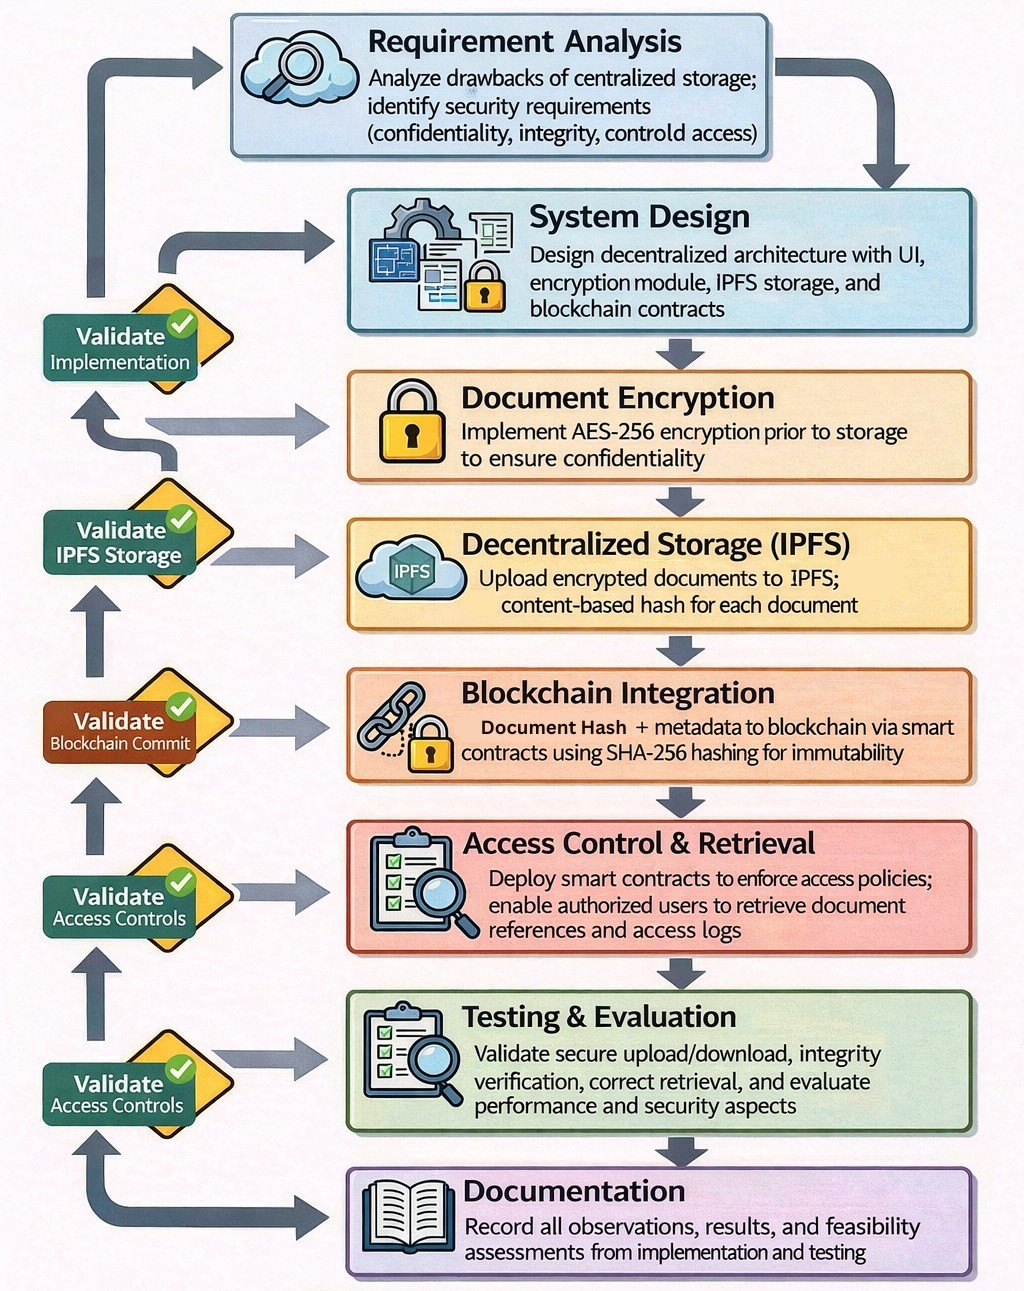
\includegraphics[width=15cm]{flowchart.jpeg}
\end{center}
\newpage
\section{Facilities required for proposed work}
The proposed system can be developed on a modern computer running Windows, macOS, or Linux, with at least 8~GB of RAM and approximately 50~GB of free disk space to accommodate development tools, node modules, and local blockchain or IPFS data. The software stack includes Node.js (version~18 or higher), npm or yarn, and Visual Studio Code (or a similar IDE with TypeScript support), along with Git for version control. The backend will use Express.js and either MongoDB or PostgreSQL as the database. Hardhat will be used for Solidity smart contract development and local Ethereum testnet simulation, while ethers.js will handle blockchain interaction. Postman or similar tools will be used for API testing. The frontend will be built using Next.js and React with TypeScript, styled using Tailwind~CSS, and will rely on the browser's built-in Web Crypto API for certain cryptographic operations and secure client-side processing. File processing will use libraries such as Mammoth.js for Word documents and PDF.js for PDF rendering, while images and text files will be handled using native browser APIs. Cryptographic operations, including SHA-256 hashing, AES-256-CBC encryption, and password hashing, will use Node.js's built-in \texttt{crypto} module together with libraries such as \texttt{bcrypt}. For blockchain and smart contract development, Hardhat, the Solidity compiler (version~0.8 or higher), and Ganache or Hardhat's built-in provider will be used to run a local blockchain network, with ethers.js handling contract deployment and interaction. Additional tools include an IPFS pinning provider such as Pinata for optional encrypted file storage, environment configuration through \texttt{.env} files, and browser developer tools for debugging client-side encryption and decryption workflows. All of these tools are available as free and open-source software.

\newpage
\section{Expected outcomes}
Upon successful completion, this project will deliver a fully functional secure document management platform that integrates end-to-end encryption using AES-256-CBC, cryptographic hashing with SHA-256, and blockchain-based integrity verification to enable secure upload, storage, sharing, and verification of sensitive documents. The system will ensure verified data integrity by storing immutable hash records within a blockchain smart contract, allowing authorized users to independently confirm that documents have not been altered since the time of upload. User privacy and confidentiality will be preserved by keeping encryption keys entirely under user control, with no plaintext data accessible to the server and only hash fingerprints recorded on the blockchain. A modern and intuitive frontend based on Next.js will provide user-friendly workflows, including secure authentication, one-click document uploads, in-browser document viewing, and simple integrity verification without requiring technical expertise. The modular and scalable system architecture will support future enhancements, while the well-documented implementation will serve as a reusable security framework for compliance-oriented applications. As a result, the project will deliver a production-ready prototype along with comprehensive documentation and deployment guidelines.

\newpage
\bibliographystyle{IEEEtran}
\bibliography{references}

\end{document}
